% Created by tikzDevice version 0.12.3.1 on 2022-09-05 08:11:28
% !TEX encoding = UTF-8 Unicode
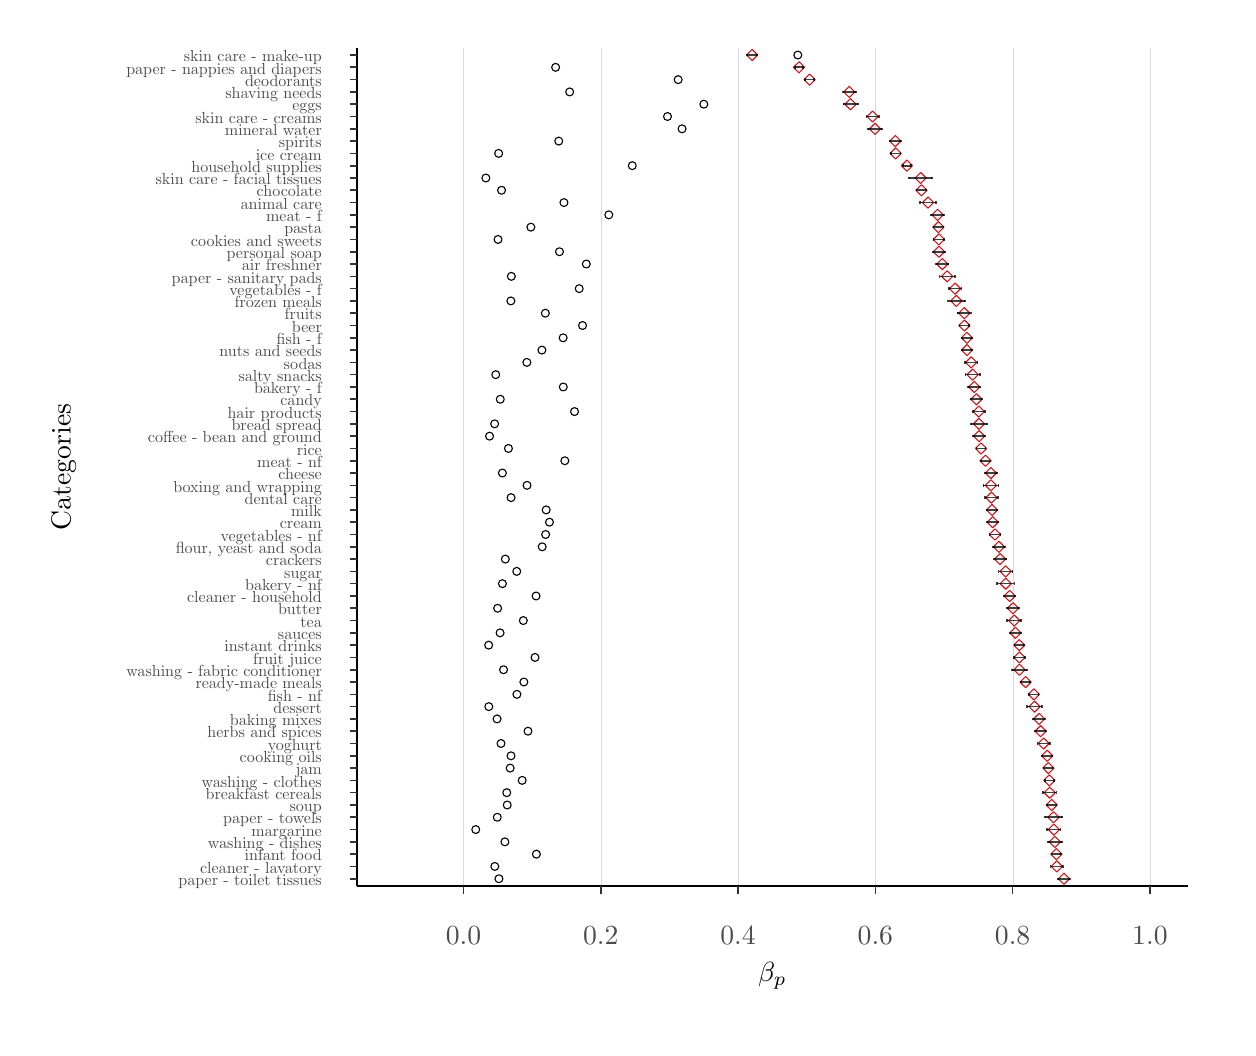
\begin{tikzpicture}[x=1pt,y=1pt]
\definecolor{fillColor}{RGB}{255,255,255}
\path[use as bounding box,fill=fillColor,fill opacity=0.00] (0,0) rectangle (433.62,361.35);
\begin{scope}
\path[clip] (  0.00,  0.00) rectangle (433.62,361.35);
\definecolor{drawColor}{RGB}{255,255,255}
\definecolor{fillColor}{RGB}{255,255,255}

\path[draw=drawColor,line width= 0.6pt,line join=round,line cap=round,fill=fillColor] (  0.00,  0.00) rectangle (433.62,361.35);
\end{scope}
\begin{scope}
\path[clip] (119.04, 51.15) rectangle (419.17,354.12);
\definecolor{drawColor}{RGB}{255,255,255}

\path[draw=drawColor,line width= 0.3pt,line join=round] (132.68, 51.15) --
	(132.68,354.12);

\path[draw=drawColor,line width= 0.3pt,line join=round] (182.29, 51.15) --
	(182.29,354.12);

\path[draw=drawColor,line width= 0.3pt,line join=round] (231.90, 51.15) --
	(231.90,354.12);

\path[draw=drawColor,line width= 0.3pt,line join=round] (281.51, 51.15) --
	(281.51,354.12);

\path[draw=drawColor,line width= 0.3pt,line join=round] (331.11, 51.15) --
	(331.11,354.12);

\path[draw=drawColor,line width= 0.3pt,line join=round] (380.72, 51.15) --
	(380.72,354.12);
\definecolor{drawColor}{gray}{0.85}

\path[draw=drawColor,line width= 0.1pt,line join=round] (157.49, 51.15) --
	(157.49,354.12);

\path[draw=drawColor,line width= 0.1pt,line join=round] (207.09, 51.15) --
	(207.09,354.12);

\path[draw=drawColor,line width= 0.1pt,line join=round] (256.70, 51.15) --
	(256.70,354.12);

\path[draw=drawColor,line width= 0.1pt,line join=round] (306.31, 51.15) --
	(306.31,354.12);

\path[draw=drawColor,line width= 0.1pt,line join=round] (355.92, 51.15) --
	(355.92,354.12);

\path[draw=drawColor,line width= 0.1pt,line join=round] (405.52, 51.15) --
	(405.52,354.12);
\definecolor{drawColor}{RGB}{0,0,0}

\path[draw=drawColor,line width= 0.4pt,line join=round,line cap=round] (201.86,275.94) circle (  1.43);

\path[draw=drawColor,line width= 0.4pt,line join=round,line cap=round] (193.78,298.15) circle (  1.43);

\path[draw=drawColor,line width= 0.4pt,line join=round,line cap=round] (193.54,231.51) circle (  1.43);

\path[draw=drawColor,line width= 0.4pt,line join=round,line cap=round] (171.55,160.44) circle (  1.43);

\path[draw=drawColor,line width= 0.4pt,line join=round,line cap=round] (169.61,111.57) circle (  1.43);

\path[draw=drawColor,line width= 0.4pt,line join=round,line cap=round] (200.50,253.73) circle (  1.43);

\path[draw=drawColor,line width= 0.4pt,line join=round,line cap=round] (180.44,195.97) circle (  1.43);

\path[draw=drawColor,line width= 0.4pt,line join=round,line cap=round] (168.73,218.19) circle (  1.43);

\path[draw=drawColor,line width= 0.4pt,line join=round,line cap=round] (173.12, 84.92) circle (  1.43);

\path[draw=drawColor,line width= 0.4pt,line join=round,line cap=round] (169.81,151.55) circle (  1.43);

\path[draw=drawColor,line width= 0.4pt,line join=round,line cap=round] (170.77,227.07) circle (  1.43);

\path[draw=drawColor,line width= 0.4pt,line join=round,line cap=round] (171.54,200.42) circle (  1.43);

\path[draw=drawColor,line width= 0.4pt,line join=round,line cap=round] (171.23,302.59) circle (  1.43);

\path[draw=drawColor,line width= 0.4pt,line join=round,line cap=round] (183.71,155.99) circle (  1.43);

\path[draw=drawColor,line width= 0.4pt,line join=round,line cap=round] (168.80, 58.26) circle (  1.43);

\path[draw=drawColor,line width= 0.4pt,line join=round,line cap=round] (166.90,213.74) circle (  1.43);

\path[draw=drawColor,line width= 0.4pt,line join=round,line cap=round] (169.96,284.82) circle (  1.43);

\path[draw=drawColor,line width= 0.4pt,line join=round,line cap=round] (174.65, 98.24) circle (  1.43);

\path[draw=drawColor,line width= 0.4pt,line join=round,line cap=round] (172.60,169.32) circle (  1.43);

\path[draw=drawColor,line width= 0.4pt,line join=round,line cap=round] (188.55,182.65) circle (  1.43);

\path[draw=drawColor,line width= 0.4pt,line join=round,line cap=round] (174.67,191.53) circle (  1.43);

\path[draw=drawColor,line width= 0.4pt,line join=round,line cap=round] (235.05,342.57) circle (  1.43);

\path[draw=drawColor,line width= 0.4pt,line join=round,line cap=round] (166.63,116.01) circle (  1.43);

\path[draw=drawColor,line width= 0.4pt,line join=round,line cap=round] (244.33,333.69) circle (  1.43);

\path[draw=drawColor,line width= 0.4pt,line join=round,line cap=round] (193.49,249.28) circle (  1.43);

\path[draw=drawColor,line width= 0.4pt,line join=round,line cap=round] (176.78,120.45) circle (  1.43);

\path[draw=drawColor,line width= 0.4pt,line join=round,line cap=round] (185.92,173.76) circle (  1.43);

\path[draw=drawColor,line width= 0.4pt,line join=round,line cap=round] (174.60,262.61) circle (  1.43);

\path[draw=drawColor,line width= 0.4pt,line join=round,line cap=round] (183.33,133.78) circle (  1.43);

\path[draw=drawColor,line width= 0.4pt,line join=round,line cap=round] (187.06,258.17) circle (  1.43);

\path[draw=drawColor,line width= 0.4pt,line join=round,line cap=round] (197.60,222.63) circle (  1.43);

\path[draw=drawColor,line width= 0.4pt,line join=round,line cap=round] (180.78,107.13) circle (  1.43);

\path[draw=drawColor,line width= 0.4pt,line join=round,line cap=round] (218.47,311.48) circle (  1.43);

\path[draw=drawColor,line width= 0.4pt,line join=round,line cap=round] (170.19,315.92) circle (  1.43);

\path[draw=drawColor,line width= 0.4pt,line join=round,line cap=round] (183.83, 62.70) circle (  1.43);

\path[draw=drawColor,line width= 0.4pt,line join=round,line cap=round] (166.58,138.22) circle (  1.43);

\path[draw=drawColor,line width= 0.4pt,line join=round,line cap=round] (174.34, 93.80) circle (  1.43);

\path[draw=drawColor,line width= 0.4pt,line join=round,line cap=round] (161.91, 71.59) circle (  1.43);

\path[draw=drawColor,line width= 0.4pt,line join=round,line cap=round] (209.99,293.71) circle (  1.43);

\path[draw=drawColor,line width= 0.4pt,line join=round,line cap=round] (194.10,204.86) circle (  1.43);

\path[draw=drawColor,line width= 0.4pt,line join=round,line cap=round] (187.36,187.09) circle (  1.43);

\path[draw=drawColor,line width= 0.4pt,line join=round,line cap=round] (236.46,324.80) circle (  1.43);

\path[draw=drawColor,line width= 0.4pt,line join=round,line cap=round] (185.81,244.84) circle (  1.43);

\path[draw=drawColor,line width= 0.4pt,line join=round,line cap=round] (190.77,347.02) circle (  1.43);

\path[draw=drawColor,line width= 0.4pt,line join=round,line cap=round] (174.77,271.49) circle (  1.43);

\path[draw=drawColor,line width= 0.4pt,line join=round,line cap=round] (170.29, 53.82) circle (  1.43);

\path[draw=drawColor,line width= 0.4pt,line join=round,line cap=round] (169.69, 76.03) circle (  1.43);

\path[draw=drawColor,line width= 0.4pt,line join=round,line cap=round] (181.83,289.26) circle (  1.43);

\path[draw=drawColor,line width= 0.4pt,line join=round,line cap=round] (192.16,280.38) circle (  1.43);

\path[draw=drawColor,line width= 0.4pt,line join=round,line cap=round] (179.29,124.90) circle (  1.43);

\path[draw=drawColor,line width= 0.4pt,line join=round,line cap=round] (173.72,209.30) circle (  1.43);

\path[draw=drawColor,line width= 0.4pt,line join=round,line cap=round] (169.14,235.96) circle (  1.43);

\path[draw=drawColor,line width= 0.4pt,line join=round,line cap=round] (170.70,142.67) circle (  1.43);

\path[draw=drawColor,line width= 0.4pt,line join=round,line cap=round] (195.85,338.13) circle (  1.43);

\path[draw=drawColor,line width= 0.4pt,line join=round,line cap=round] (231.20,329.25) circle (  1.43);

\path[draw=drawColor,line width= 0.4pt,line join=round,line cap=round] (165.56,307.03) circle (  1.43);

\path[draw=drawColor,line width= 0.4pt,line join=round,line cap=round] (278.29,351.46) circle (  1.43);

\path[draw=drawColor,line width= 0.4pt,line join=round,line cap=round] (180.38,240.40) circle (  1.43);

\path[draw=drawColor,line width= 0.4pt,line join=round,line cap=round] (173.29, 80.47) circle (  1.43);

\path[draw=drawColor,line width= 0.4pt,line join=round,line cap=round] (191.90,320.36) circle (  1.43);

\path[draw=drawColor,line width= 0.4pt,line join=round,line cap=round] (176.72,164.88) circle (  1.43);

\path[draw=drawColor,line width= 0.4pt,line join=round,line cap=round] (179.10,147.11) circle (  1.43);

\path[draw=drawColor,line width= 0.4pt,line join=round,line cap=round] (199.29,267.05) circle (  1.43);

\path[draw=drawColor,line width= 0.4pt,line join=round,line cap=round] (187.16,178.21) circle (  1.43);

\path[draw=drawColor,line width= 0.4pt,line join=round,line cap=round] (178.69, 89.36) circle (  1.43);

\path[draw=drawColor,line width= 0.4pt,line join=round,line cap=round] (172.45, 67.15) circle (  1.43);

\path[draw=drawColor,line width= 0.4pt,line join=round,line cap=round] (171.95,129.34) circle (  1.43);

\path[draw=drawColor,line width= 0.4pt,line join=round,line cap=round] (171.03,102.69) circle (  1.43);
\definecolor{drawColor}{RGB}{203,24,29}

\path[draw=drawColor,line width= 0.4pt,line join=round,line cap=round] (328.51,275.94) --
	(330.53,277.95) --
	(332.55,275.94) --
	(330.53,273.92) --
	cycle;

\path[draw=drawColor,line width= 0.4pt,line join=round,line cap=round] (323.33,298.15) --
	(325.35,300.17) --
	(327.37,298.15) --
	(325.35,296.13) --
	cycle;

\path[draw=drawColor,line width= 0.4pt,line join=round,line cap=round] (340.03,231.51) --
	(342.05,233.53) --
	(344.07,231.51) --
	(342.05,229.50) --
	cycle;

\path[draw=drawColor,line width= 0.4pt,line join=round,line cap=round] (351.40,160.44) --
	(353.42,162.45) --
	(355.44,160.44) --
	(353.42,158.42) --
	cycle;

\path[draw=drawColor,line width= 0.4pt,line join=round,line cap=round] (363.48,111.57) --
	(365.50,113.59) --
	(367.51,111.57) --
	(365.50,109.55) --
	cycle;

\path[draw=drawColor,line width= 0.4pt,line join=round,line cap=round] (336.48,253.73) --
	(338.50,255.74) --
	(340.51,253.73) --
	(338.50,251.71) --
	cycle;

\path[draw=drawColor,line width= 0.4pt,line join=round,line cap=round] (346.05,195.97) --
	(348.07,197.99) --
	(350.09,195.97) --
	(348.07,193.96) --
	cycle;

\path[draw=drawColor,line width= 0.4pt,line join=round,line cap=round] (341.73,218.19) --
	(343.75,220.20) --
	(345.76,218.19) --
	(343.75,216.17) --
	cycle;

\path[draw=drawColor,line width= 0.4pt,line join=round,line cap=round] (367.30, 84.92) --
	(369.32, 86.93) --
	(371.33, 84.92) --
	(369.32, 82.90) --
	cycle;

\path[draw=drawColor,line width= 0.4pt,line join=round,line cap=round] (354.05,151.55) --
	(356.06,153.57) --
	(358.08,151.55) --
	(356.06,149.53) --
	cycle;

\path[draw=drawColor,line width= 0.4pt,line join=round,line cap=round] (340.81,227.07) --
	(342.82,229.09) --
	(344.84,227.07) --
	(342.82,225.05) --
	cycle;

\path[draw=drawColor,line width= 0.4pt,line join=round,line cap=round] (346.04,200.42) --
	(348.06,202.43) --
	(350.08,200.42) --
	(348.06,198.40) --
	cycle;

\path[draw=drawColor,line width= 0.4pt,line join=round,line cap=round] (320.95,302.59) --
	(322.97,304.61) --
	(324.99,302.59) --
	(322.97,300.57) --
	cycle;

\path[draw=drawColor,line width= 0.4pt,line join=round,line cap=round] (352.83,155.99) --
	(354.85,158.01) --
	(356.87,155.99) --
	(354.85,153.98) --
	cycle;

\path[draw=drawColor,line width= 0.4pt,line join=round,line cap=round] (369.87, 58.26) --
	(371.88, 60.28) --
	(373.90, 58.26) --
	(371.88, 56.24) --
	cycle;

\path[draw=drawColor,line width= 0.4pt,line join=round,line cap=round] (341.76,213.74) --
	(343.78,215.76) --
	(345.80,213.74) --
	(343.78,211.73) --
	cycle;

\path[draw=drawColor,line width= 0.4pt,line join=round,line cap=round] (327.25,284.82) --
	(329.27,286.84) --
	(331.29,284.82) --
	(329.27,282.80) --
	cycle;

\path[draw=drawColor,line width= 0.4pt,line join=round,line cap=round] (366.39, 98.24) --
	(368.40,100.26) --
	(370.42, 98.24) --
	(368.40, 96.23) --
	cycle;

\path[draw=drawColor,line width= 0.4pt,line join=round,line cap=round] (349.34,169.32) --
	(351.36,171.34) --
	(353.37,169.32) --
	(351.36,167.30) --
	cycle;

\path[draw=drawColor,line width= 0.4pt,line join=round,line cap=round] (346.71,182.65) --
	(348.72,184.67) --
	(350.74,182.65) --
	(348.72,180.63) --
	cycle;

\path[draw=drawColor,line width= 0.4pt,line join=round,line cap=round] (346.24,191.53) --
	(348.26,193.55) --
	(350.28,191.53) --
	(348.26,189.51) --
	cycle;

\path[draw=drawColor,line width= 0.4pt,line join=round,line cap=round] (280.53,342.57) --
	(282.55,344.59) --
	(284.56,342.57) --
	(282.55,340.56) --
	cycle;

\path[draw=drawColor,line width= 0.4pt,line join=round,line cap=round] (361.80,116.01) --
	(363.82,118.03) --
	(365.84,116.01) --
	(363.82,113.99) --
	cycle;

\path[draw=drawColor,line width= 0.4pt,line join=round,line cap=round] (295.32,333.69) --
	(297.33,335.71) --
	(299.35,333.69) --
	(297.33,331.67) --
	cycle;

\path[draw=drawColor,line width= 0.4pt,line join=round,line cap=round] (337.37,249.28) --
	(339.39,251.30) --
	(341.40,249.28) --
	(339.39,247.27) --
	cycle;

\path[draw=drawColor,line width= 0.4pt,line join=round,line cap=round] (361.58,120.45) --
	(363.60,122.47) --
	(365.62,120.45) --
	(363.60,118.44) --
	cycle;

\path[draw=drawColor,line width= 0.4pt,line join=round,line cap=round] (348.97,173.76) --
	(350.98,175.78) --
	(353.00,173.76) --
	(350.98,171.75) --
	cycle;

\path[draw=drawColor,line width= 0.4pt,line join=round,line cap=round] (333.55,262.61) --
	(335.57,264.63) --
	(337.58,262.61) --
	(335.57,260.59) --
	cycle;

\path[draw=drawColor,line width= 0.4pt,line join=round,line cap=round] (356.35,133.78) --
	(358.37,135.80) --
	(360.38,133.78) --
	(358.37,131.76) --
	cycle;

\path[draw=drawColor,line width= 0.4pt,line join=round,line cap=round] (336.44,258.17) --
	(338.46,260.19) --
	(340.48,258.17) --
	(338.46,256.15) --
	cycle;

\path[draw=drawColor,line width= 0.4pt,line join=round,line cap=round] (341.67,222.63) --
	(343.69,224.65) --
	(345.71,222.63) --
	(343.69,220.61) --
	cycle;

\path[draw=drawColor,line width= 0.4pt,line join=round,line cap=round] (364.00,107.13) --
	(366.02,109.14) --
	(368.04,107.13) --
	(366.02,105.11) --
	cycle;

\path[draw=drawColor,line width= 0.4pt,line join=round,line cap=round] (315.68,311.48) --
	(317.70,313.49) --
	(319.72,311.48) --
	(317.70,309.46) --
	cycle;

\path[draw=drawColor,line width= 0.4pt,line join=round,line cap=round] (311.63,315.92) --
	(313.65,317.94) --
	(315.67,315.92) --
	(313.65,313.90) --
	cycle;

\path[draw=drawColor,line width= 0.4pt,line join=round,line cap=round] (369.70, 62.70) --
	(371.71, 64.72) --
	(373.73, 62.70) --
	(371.71, 60.69) --
	cycle;

\path[draw=drawColor,line width= 0.4pt,line join=round,line cap=round] (356.29,138.22) --
	(358.31,140.24) --
	(360.32,138.22) --
	(358.31,136.21) --
	cycle;

\path[draw=drawColor,line width= 0.4pt,line join=round,line cap=round] (366.84, 93.80) --
	(368.85, 95.82) --
	(370.87, 93.80) --
	(368.85, 91.78) --
	cycle;

\path[draw=drawColor,line width= 0.4pt,line join=round,line cap=round] (368.80, 71.59) --
	(370.82, 73.61) --
	(372.84, 71.59) --
	(370.82, 69.57) --
	cycle;

\path[draw=drawColor,line width= 0.4pt,line join=round,line cap=round] (326.80,293.71) --
	(328.81,295.72) --
	(330.83,293.71) --
	(328.81,291.69) --
	cycle;

\path[draw=drawColor,line width= 0.4pt,line join=round,line cap=round] (344.10,204.86) --
	(346.12,206.88) --
	(348.14,204.86) --
	(346.12,202.84) --
	cycle;

\path[draw=drawColor,line width= 0.4pt,line join=round,line cap=round] (346.45,187.09) --
	(348.47,189.11) --
	(350.48,187.09) --
	(348.47,185.07) --
	cycle;

\path[draw=drawColor,line width= 0.4pt,line join=round,line cap=round] (304.16,324.80) --
	(306.18,326.82) --
	(308.19,324.80) --
	(306.18,322.79) --
	cycle;

\path[draw=drawColor,line width= 0.4pt,line join=round,line cap=round] (337.39,244.84) --
	(339.41,246.86) --
	(341.42,244.84) --
	(339.41,242.82) --
	cycle;

\path[draw=drawColor,line width= 0.4pt,line join=round,line cap=round] (276.71,347.02) --
	(278.73,349.03) --
	(280.75,347.02) --
	(278.73,345.00) --
	cycle;

\path[draw=drawColor,line width= 0.4pt,line join=round,line cap=round] (330.24,271.49) --
	(332.26,273.51) --
	(334.28,271.49) --
	(332.26,269.48) --
	cycle;

\path[draw=drawColor,line width= 0.4pt,line join=round,line cap=round] (372.44, 53.82) --
	(374.46, 55.84) --
	(376.47, 53.82) --
	(374.46, 51.80) --
	cycle;

\path[draw=drawColor,line width= 0.4pt,line join=round,line cap=round] (368.66, 76.03) --
	(370.67, 78.05) --
	(372.69, 76.03) --
	(370.67, 74.01) --
	cycle;

\path[draw=drawColor,line width= 0.4pt,line join=round,line cap=round] (327.08,289.26) --
	(329.10,291.28) --
	(331.11,289.26) --
	(329.10,287.25) --
	cycle;

\path[draw=drawColor,line width= 0.4pt,line join=round,line cap=round] (327.27,280.38) --
	(329.28,282.40) --
	(331.30,280.38) --
	(329.28,278.36) --
	cycle;

\path[draw=drawColor,line width= 0.4pt,line join=round,line cap=round] (358.58,124.90) --
	(360.60,126.91) --
	(362.62,124.90) --
	(360.60,122.88) --
	cycle;

\path[draw=drawColor,line width= 0.4pt,line join=round,line cap=round] (342.49,209.30) --
	(344.50,211.32) --
	(346.52,209.30) --
	(344.50,207.28) --
	cycle;

\path[draw=drawColor,line width= 0.4pt,line join=round,line cap=round] (339.46,235.96) --
	(341.47,237.97) --
	(343.49,235.96) --
	(341.47,233.94) --
	cycle;

\path[draw=drawColor,line width= 0.4pt,line join=round,line cap=round] (354.89,142.67) --
	(356.91,144.68) --
	(358.93,142.67) --
	(356.91,140.65) --
	cycle;

\path[draw=drawColor,line width= 0.4pt,line join=round,line cap=round] (294.87,338.13) --
	(296.89,340.15) --
	(298.90,338.13) --
	(296.89,336.11) --
	cycle;

\path[draw=drawColor,line width= 0.4pt,line join=round,line cap=round] (303.30,329.25) --
	(305.32,331.26) --
	(307.33,329.25) --
	(305.32,327.23) --
	cycle;

\path[draw=drawColor,line width= 0.4pt,line join=round,line cap=round] (320.65,307.03) --
	(322.67,309.05) --
	(324.69,307.03) --
	(322.67,305.02) --
	cycle;

\path[draw=drawColor,line width= 0.4pt,line join=round,line cap=round] (259.77,351.46) --
	(261.79,353.48) --
	(263.81,351.46) --
	(261.79,349.44) --
	cycle;

\path[draw=drawColor,line width= 0.4pt,line join=round,line cap=round] (338.91,240.40) --
	(340.93,242.42) --
	(342.95,240.40) --
	(340.93,238.38) --
	cycle;

\path[draw=drawColor,line width= 0.4pt,line join=round,line cap=round] (368.00, 80.47) --
	(370.02, 82.49) --
	(372.04, 80.47) --
	(370.02, 78.46) --
	cycle;

\path[draw=drawColor,line width= 0.4pt,line join=round,line cap=round] (311.50,320.36) --
	(313.51,322.38) --
	(315.53,320.36) --
	(313.51,318.34) --
	cycle;

\path[draw=drawColor,line width= 0.4pt,line join=round,line cap=round] (351.35,164.88) --
	(353.36,166.90) --
	(355.38,164.88) --
	(353.36,162.86) --
	cycle;

\path[draw=drawColor,line width= 0.4pt,line join=round,line cap=round] (354.48,147.11) --
	(356.49,149.13) --
	(358.51,147.11) --
	(356.49,145.09) --
	cycle;

\path[draw=drawColor,line width= 0.4pt,line join=round,line cap=round] (333.08,267.05) --
	(335.10,269.07) --
	(337.12,267.05) --
	(335.10,265.04) --
	cycle;

\path[draw=drawColor,line width= 0.4pt,line join=round,line cap=round] (347.52,178.21) --
	(349.54,180.22) --
	(351.56,178.21) --
	(349.54,176.19) --
	cycle;

\path[draw=drawColor,line width= 0.4pt,line join=round,line cap=round] (367.17, 89.36) --
	(369.19, 91.38) --
	(371.20, 89.36) --
	(369.19, 87.34) --
	cycle;

\path[draw=drawColor,line width= 0.4pt,line join=round,line cap=round] (369.16, 67.15) --
	(371.18, 69.16) --
	(373.19, 67.15) --
	(371.18, 65.13) --
	cycle;

\path[draw=drawColor,line width= 0.4pt,line join=round,line cap=round] (356.38,129.34) --
	(358.39,131.36) --
	(360.41,129.34) --
	(358.39,127.32) --
	cycle;

\path[draw=drawColor,line width= 0.4pt,line join=round,line cap=round] (365.11,102.69) --
	(367.12,104.70) --
	(369.14,102.69) --
	(367.12,100.67) --
	cycle;
\definecolor{drawColor}{RGB}{0,0,0}

\path[draw=drawColor,draw opacity=0.75,line width= 0.6pt,line join=round] (332.76,275.49) --
	(332.76,276.38);

\path[draw=drawColor,draw opacity=0.75,line width= 0.6pt,line join=round] (332.76,275.94) --
	(328.30,275.94);

\path[draw=drawColor,draw opacity=0.75,line width= 0.6pt,line join=round] (328.30,275.49) --
	(328.30,276.38);

\path[draw=drawColor,draw opacity=0.75,line width= 0.6pt,line join=round] (328.16,297.70) --
	(328.16,298.59);

\path[draw=drawColor,draw opacity=0.75,line width= 0.6pt,line join=round] (328.16,298.15) --
	(322.54,298.15);

\path[draw=drawColor,draw opacity=0.75,line width= 0.6pt,line join=round] (322.54,297.70) --
	(322.54,298.59);

\path[draw=drawColor,draw opacity=0.75,line width= 0.6pt,line join=round] (344.29,231.07) --
	(344.29,231.96);

\path[draw=drawColor,draw opacity=0.75,line width= 0.6pt,line join=round] (344.29,231.51) --
	(339.81,231.51);

\path[draw=drawColor,draw opacity=0.75,line width= 0.6pt,line join=round] (339.81,231.07) --
	(339.81,231.96);

\path[draw=drawColor,draw opacity=0.75,line width= 0.6pt,line join=round] (356.53,159.99) --
	(356.53,160.88);

\path[draw=drawColor,draw opacity=0.75,line width= 0.6pt,line join=round] (356.53,160.44) --
	(350.31,160.44);

\path[draw=drawColor,draw opacity=0.75,line width= 0.6pt,line join=round] (350.31,159.99) --
	(350.31,160.88);

\path[draw=drawColor,draw opacity=0.75,line width= 0.6pt,line join=round] (367.78,111.13) --
	(367.78,112.01);

\path[draw=drawColor,draw opacity=0.75,line width= 0.6pt,line join=round] (367.78,111.57) --
	(363.21,111.57);

\path[draw=drawColor,draw opacity=0.75,line width= 0.6pt,line join=round] (363.21,111.13) --
	(363.21,112.01);

\path[draw=drawColor,draw opacity=0.75,line width= 0.6pt,line join=round] (340.22,253.28) --
	(340.22,254.17);

\path[draw=drawColor,draw opacity=0.75,line width= 0.6pt,line join=round] (340.22,253.73) --
	(336.77,253.73);

\path[draw=drawColor,draw opacity=0.75,line width= 0.6pt,line join=round] (336.77,253.28) --
	(336.77,254.17);

\path[draw=drawColor,draw opacity=0.75,line width= 0.6pt,line join=round] (350.81,195.53) --
	(350.81,196.42);

\path[draw=drawColor,draw opacity=0.75,line width= 0.6pt,line join=round] (350.81,195.97) --
	(345.34,195.97);

\path[draw=drawColor,draw opacity=0.75,line width= 0.6pt,line join=round] (345.34,195.53) --
	(345.34,196.42);

\path[draw=drawColor,draw opacity=0.75,line width= 0.6pt,line join=round] (346.66,217.74) --
	(346.66,218.63);

\path[draw=drawColor,draw opacity=0.75,line width= 0.6pt,line join=round] (346.66,218.19) --
	(340.83,218.19);

\path[draw=drawColor,draw opacity=0.75,line width= 0.6pt,line join=round] (340.83,217.74) --
	(340.83,218.63);

\path[draw=drawColor,draw opacity=0.75,line width= 0.6pt,line join=round] (371.74, 84.47) --
	(371.74, 85.36);

\path[draw=drawColor,draw opacity=0.75,line width= 0.6pt,line join=round] (371.74, 84.92) --
	(366.89, 84.92);

\path[draw=drawColor,draw opacity=0.75,line width= 0.6pt,line join=round] (366.89, 84.47) --
	(366.89, 85.36);

\path[draw=drawColor,draw opacity=0.75,line width= 0.6pt,line join=round] (358.25,151.11) --
	(358.25,152.00);

\path[draw=drawColor,draw opacity=0.75,line width= 0.6pt,line join=round] (358.25,151.55) --
	(353.88,151.55);

\path[draw=drawColor,draw opacity=0.75,line width= 0.6pt,line join=round] (353.88,151.11) --
	(353.88,152.00);

\path[draw=drawColor,draw opacity=0.75,line width= 0.6pt,line join=round] (344.96,226.63) --
	(344.96,227.52);

\path[draw=drawColor,draw opacity=0.75,line width= 0.6pt,line join=round] (344.96,227.07) --
	(340.68,227.07);

\path[draw=drawColor,draw opacity=0.75,line width= 0.6pt,line join=round] (340.68,226.63) --
	(340.68,227.52);

\path[draw=drawColor,draw opacity=0.75,line width= 0.6pt,line join=round] (350.20,199.97) --
	(350.20,200.86);

\path[draw=drawColor,draw opacity=0.75,line width= 0.6pt,line join=round] (350.20,200.42) --
	(345.93,200.42);

\path[draw=drawColor,draw opacity=0.75,line width= 0.6pt,line join=round] (345.93,199.97) --
	(345.93,200.86);

\path[draw=drawColor,draw opacity=0.75,line width= 0.6pt,line join=round] (324.81,302.15) --
	(324.81,303.04);

\path[draw=drawColor,draw opacity=0.75,line width= 0.6pt,line join=round] (324.81,302.59) --
	(321.14,302.59);

\path[draw=drawColor,draw opacity=0.75,line width= 0.6pt,line join=round] (321.14,302.15) --
	(321.14,303.04);

\path[draw=drawColor,draw opacity=0.75,line width= 0.6pt,line join=round] (356.88,155.55) --
	(356.88,156.44);

\path[draw=drawColor,draw opacity=0.75,line width= 0.6pt,line join=round] (356.88,155.99) --
	(352.82,155.99);

\path[draw=drawColor,draw opacity=0.75,line width= 0.6pt,line join=round] (352.82,155.55) --
	(352.82,156.44);

\path[draw=drawColor,draw opacity=0.75,line width= 0.6pt,line join=round] (374.16, 57.82) --
	(374.16, 58.71);

\path[draw=drawColor,draw opacity=0.75,line width= 0.6pt,line join=round] (374.16, 58.26) --
	(369.60, 58.26);

\path[draw=drawColor,draw opacity=0.75,line width= 0.6pt,line join=round] (369.60, 57.82) --
	(369.60, 58.71);

\path[draw=drawColor,draw opacity=0.75,line width= 0.6pt,line join=round] (345.97,213.30) --
	(345.97,214.19);

\path[draw=drawColor,draw opacity=0.75,line width= 0.6pt,line join=round] (345.97,213.74) --
	(341.60,213.74);

\path[draw=drawColor,draw opacity=0.75,line width= 0.6pt,line join=round] (341.60,213.30) --
	(341.60,214.19);

\path[draw=drawColor,draw opacity=0.75,line width= 0.6pt,line join=round] (331.19,284.38) --
	(331.19,285.27);

\path[draw=drawColor,draw opacity=0.75,line width= 0.6pt,line join=round] (331.19,284.82) --
	(327.35,284.82);

\path[draw=drawColor,draw opacity=0.75,line width= 0.6pt,line join=round] (327.35,284.38) --
	(327.35,285.27);

\path[draw=drawColor,draw opacity=0.75,line width= 0.6pt,line join=round] (370.35, 97.80) --
	(370.35, 98.69);

\path[draw=drawColor,draw opacity=0.75,line width= 0.6pt,line join=round] (370.35, 98.24) --
	(366.46, 98.24);

\path[draw=drawColor,draw opacity=0.75,line width= 0.6pt,line join=round] (366.46, 97.80) --
	(366.46, 98.69);

\path[draw=drawColor,draw opacity=0.75,line width= 0.6pt,line join=round] (353.70,168.88) --
	(353.70,169.76);

\path[draw=drawColor,draw opacity=0.75,line width= 0.6pt,line join=round] (353.70,169.32) --
	(349.01,169.32);

\path[draw=drawColor,draw opacity=0.75,line width= 0.6pt,line join=round] (349.01,168.88) --
	(349.01,169.76);

\path[draw=drawColor,draw opacity=0.75,line width= 0.6pt,line join=round] (350.86,182.20) --
	(350.86,183.09);

\path[draw=drawColor,draw opacity=0.75,line width= 0.6pt,line join=round] (350.86,182.65) --
	(346.59,182.65);

\path[draw=drawColor,draw opacity=0.75,line width= 0.6pt,line join=round] (346.59,182.20) --
	(346.59,183.09);

\path[draw=drawColor,draw opacity=0.75,line width= 0.6pt,line join=round] (350.54,191.09) --
	(350.54,191.98);

\path[draw=drawColor,draw opacity=0.75,line width= 0.6pt,line join=round] (350.54,191.53) --
	(345.98,191.53);

\path[draw=drawColor,draw opacity=0.75,line width= 0.6pt,line join=round] (345.98,191.09) --
	(345.98,191.98);

\path[draw=drawColor,draw opacity=0.75,line width= 0.6pt,line join=round] (284.20,342.13) --
	(284.20,343.02);

\path[draw=drawColor,draw opacity=0.75,line width= 0.6pt,line join=round] (284.20,342.57) --
	(280.89,342.57);

\path[draw=drawColor,draw opacity=0.75,line width= 0.6pt,line join=round] (280.89,342.13) --
	(280.89,343.02);

\path[draw=drawColor,draw opacity=0.75,line width= 0.6pt,line join=round] (366.57,115.57) --
	(366.57,116.46);

\path[draw=drawColor,draw opacity=0.75,line width= 0.6pt,line join=round] (366.57,116.01) --
	(361.07,116.01);

\path[draw=drawColor,draw opacity=0.75,line width= 0.6pt,line join=round] (361.07,115.57) --
	(361.07,116.46);

\path[draw=drawColor,draw opacity=0.75,line width= 0.6pt,line join=round] (299.92,333.24) --
	(299.92,334.13);

\path[draw=drawColor,draw opacity=0.75,line width= 0.6pt,line join=round] (299.92,333.69) --
	(294.75,333.69);

\path[draw=drawColor,draw opacity=0.75,line width= 0.6pt,line join=round] (294.75,333.24) --
	(294.75,334.13);

\path[draw=drawColor,draw opacity=0.75,line width= 0.6pt,line join=round] (341.30,248.84) --
	(341.30,249.73);

\path[draw=drawColor,draw opacity=0.75,line width= 0.6pt,line join=round] (341.30,249.28) --
	(337.47,249.28);

\path[draw=drawColor,draw opacity=0.75,line width= 0.6pt,line join=round] (337.47,248.84) --
	(337.47,249.73);

\path[draw=drawColor,draw opacity=0.75,line width= 0.6pt,line join=round] (365.27,120.01) --
	(365.27,120.90);

\path[draw=drawColor,draw opacity=0.75,line width= 0.6pt,line join=round] (365.27,120.45) --
	(361.93,120.45);

\path[draw=drawColor,draw opacity=0.75,line width= 0.6pt,line join=round] (361.93,120.01) --
	(361.93,120.90);

\path[draw=drawColor,draw opacity=0.75,line width= 0.6pt,line join=round] (353.24,173.32) --
	(353.24,174.21);

\path[draw=drawColor,draw opacity=0.75,line width= 0.6pt,line join=round] (353.24,173.76) --
	(348.73,173.76);

\path[draw=drawColor,draw opacity=0.75,line width= 0.6pt,line join=round] (348.73,173.32) --
	(348.73,174.21);

\path[draw=drawColor,draw opacity=0.75,line width= 0.6pt,line join=round] (338.74,262.17) --
	(338.74,263.05);

\path[draw=drawColor,draw opacity=0.75,line width= 0.6pt,line join=round] (338.74,262.61) --
	(332.40,262.61);

\path[draw=drawColor,draw opacity=0.75,line width= 0.6pt,line join=round] (332.40,262.17) --
	(332.40,263.05);

\path[draw=drawColor,draw opacity=0.75,line width= 0.6pt,line join=round] (360.36,133.34) --
	(360.36,134.23);

\path[draw=drawColor,draw opacity=0.75,line width= 0.6pt,line join=round] (360.36,133.78) --
	(356.37,133.78);

\path[draw=drawColor,draw opacity=0.75,line width= 0.6pt,line join=round] (356.37,133.34) --
	(356.37,134.23);

\path[draw=drawColor,draw opacity=0.75,line width= 0.6pt,line join=round] (340.99,257.72) --
	(340.99,258.61);

\path[draw=drawColor,draw opacity=0.75,line width= 0.6pt,line join=round] (340.99,258.17) --
	(335.93,258.17);

\path[draw=drawColor,draw opacity=0.75,line width= 0.6pt,line join=round] (335.93,257.72) --
	(335.93,258.61);

\path[draw=drawColor,draw opacity=0.75,line width= 0.6pt,line join=round] (345.86,222.18) --
	(345.86,223.07);

\path[draw=drawColor,draw opacity=0.75,line width= 0.6pt,line join=round] (345.86,222.63) --
	(341.52,222.63);

\path[draw=drawColor,draw opacity=0.75,line width= 0.6pt,line join=round] (341.52,222.18) --
	(341.52,223.07);

\path[draw=drawColor,draw opacity=0.75,line width= 0.6pt,line join=round] (368.11,106.68) --
	(368.11,107.57);

\path[draw=drawColor,draw opacity=0.75,line width= 0.6pt,line join=round] (368.11,107.13) --
	(363.92,107.13);

\path[draw=drawColor,draw opacity=0.75,line width= 0.6pt,line join=round] (363.92,106.68) --
	(363.92,107.57);

\path[draw=drawColor,draw opacity=0.75,line width= 0.6pt,line join=round] (319.16,311.03) --
	(319.16,311.92);

\path[draw=drawColor,draw opacity=0.75,line width= 0.6pt,line join=round] (319.16,311.48) --
	(316.23,311.48);

\path[draw=drawColor,draw opacity=0.75,line width= 0.6pt,line join=round] (316.23,311.03) --
	(316.23,311.92);

\path[draw=drawColor,draw opacity=0.75,line width= 0.6pt,line join=round] (315.35,315.47) --
	(315.35,316.36);

\path[draw=drawColor,draw opacity=0.75,line width= 0.6pt,line join=round] (315.35,315.92) --
	(311.95,315.92);

\path[draw=drawColor,draw opacity=0.75,line width= 0.6pt,line join=round] (311.95,315.47) --
	(311.95,316.36);

\path[draw=drawColor,draw opacity=0.75,line width= 0.6pt,line join=round] (373.42, 62.26) --
	(373.42, 63.15);

\path[draw=drawColor,draw opacity=0.75,line width= 0.6pt,line join=round] (373.42, 62.70) --
	(370.01, 62.70);

\path[draw=drawColor,draw opacity=0.75,line width= 0.6pt,line join=round] (370.01, 62.26) --
	(370.01, 63.15);

\path[draw=drawColor,draw opacity=0.75,line width= 0.6pt,line join=round] (360.03,137.78) --
	(360.03,138.67);

\path[draw=drawColor,draw opacity=0.75,line width= 0.6pt,line join=round] (360.03,138.22) --
	(356.58,138.22);

\path[draw=drawColor,draw opacity=0.75,line width= 0.6pt,line join=round] (356.58,137.78) --
	(356.58,138.67);

\path[draw=drawColor,draw opacity=0.75,line width= 0.6pt,line join=round] (370.65, 93.36) --
	(370.65, 94.24);

\path[draw=drawColor,draw opacity=0.75,line width= 0.6pt,line join=round] (370.65, 93.80) --
	(367.06, 93.80);

\path[draw=drawColor,draw opacity=0.75,line width= 0.6pt,line join=round] (367.06, 93.36) --
	(367.06, 94.24);

\path[draw=drawColor,draw opacity=0.75,line width= 0.6pt,line join=round] (373.25, 71.14) --
	(373.25, 72.03);

\path[draw=drawColor,draw opacity=0.75,line width= 0.6pt,line join=round] (373.25, 71.59) --
	(368.39, 71.59);

\path[draw=drawColor,draw opacity=0.75,line width= 0.6pt,line join=round] (368.39, 71.14) --
	(368.39, 72.03);

\path[draw=drawColor,draw opacity=0.75,line width= 0.6pt,line join=round] (331.17,293.26) --
	(331.17,294.15);

\path[draw=drawColor,draw opacity=0.75,line width= 0.6pt,line join=round] (331.17,293.71) --
	(326.46,293.71);

\path[draw=drawColor,draw opacity=0.75,line width= 0.6pt,line join=round] (326.46,293.26) --
	(326.46,294.15);

\path[draw=drawColor,draw opacity=0.75,line width= 0.6pt,line join=round] (347.88,204.42) --
	(347.88,205.30);

\path[draw=drawColor,draw opacity=0.75,line width= 0.6pt,line join=round] (347.88,204.86) --
	(344.37,204.86);

\path[draw=drawColor,draw opacity=0.75,line width= 0.6pt,line join=round] (344.37,204.42) --
	(344.37,205.30);

\path[draw=drawColor,draw opacity=0.75,line width= 0.6pt,line join=round] (350.50,186.65) --
	(350.50,187.53);

\path[draw=drawColor,draw opacity=0.75,line width= 0.6pt,line join=round] (350.50,187.09) --
	(346.43,187.09);

\path[draw=drawColor,draw opacity=0.75,line width= 0.6pt,line join=round] (346.43,186.65) --
	(346.43,187.53);

\path[draw=drawColor,draw opacity=0.75,line width= 0.6pt,line join=round] (308.79,324.36) --
	(308.79,325.25);

\path[draw=drawColor,draw opacity=0.75,line width= 0.6pt,line join=round] (308.79,324.80) --
	(303.56,324.80);

\path[draw=drawColor,draw opacity=0.75,line width= 0.6pt,line join=round] (303.56,324.36) --
	(303.56,325.25);

\path[draw=drawColor,draw opacity=0.75,line width= 0.6pt,line join=round] (341.20,244.40) --
	(341.20,245.29);

\path[draw=drawColor,draw opacity=0.75,line width= 0.6pt,line join=round] (341.20,244.84) --
	(337.61,244.84);

\path[draw=drawColor,draw opacity=0.75,line width= 0.6pt,line join=round] (337.61,244.40) --
	(337.61,245.29);

\path[draw=drawColor,draw opacity=0.75,line width= 0.6pt,line join=round] (280.19,346.57) --
	(280.19,347.46);

\path[draw=drawColor,draw opacity=0.75,line width= 0.6pt,line join=round] (280.19,347.02) --
	(277.27,347.02);

\path[draw=drawColor,draw opacity=0.75,line width= 0.6pt,line join=round] (277.27,346.57) --
	(277.27,347.46);

\path[draw=drawColor,draw opacity=0.75,line width= 0.6pt,line join=round] (335.01,271.05) --
	(335.01,271.94);

\path[draw=drawColor,draw opacity=0.75,line width= 0.6pt,line join=round] (335.01,271.49) --
	(329.51,271.49);

\path[draw=drawColor,draw opacity=0.75,line width= 0.6pt,line join=round] (329.51,271.05) --
	(329.51,271.94);

\path[draw=drawColor,draw opacity=0.75,line width= 0.6pt,line join=round] (376.54, 53.37) --
	(376.54, 54.26);

\path[draw=drawColor,draw opacity=0.75,line width= 0.6pt,line join=round] (376.54, 53.82) --
	(372.38, 53.82);

\path[draw=drawColor,draw opacity=0.75,line width= 0.6pt,line join=round] (372.38, 53.37) --
	(372.38, 54.26);

\path[draw=drawColor,draw opacity=0.75,line width= 0.6pt,line join=round] (373.64, 75.59) --
	(373.64, 76.48);

\path[draw=drawColor,draw opacity=0.75,line width= 0.6pt,line join=round] (373.64, 76.03) --
	(367.71, 76.03);

\path[draw=drawColor,draw opacity=0.75,line width= 0.6pt,line join=round] (367.71, 75.59) --
	(367.71, 76.48);

\path[draw=drawColor,draw opacity=0.75,line width= 0.6pt,line join=round] (330.90,288.82) --
	(330.90,289.71);

\path[draw=drawColor,draw opacity=0.75,line width= 0.6pt,line join=round] (330.90,289.26) --
	(327.29,289.26);

\path[draw=drawColor,draw opacity=0.75,line width= 0.6pt,line join=round] (327.29,288.82) --
	(327.29,289.71);

\path[draw=drawColor,draw opacity=0.75,line width= 0.6pt,line join=round] (331.46,279.94) --
	(331.46,280.82);

\path[draw=drawColor,draw opacity=0.75,line width= 0.6pt,line join=round] (331.46,280.38) --
	(327.11,280.38);

\path[draw=drawColor,draw opacity=0.75,line width= 0.6pt,line join=round] (327.11,279.94) --
	(327.11,280.82);

\path[draw=drawColor,draw opacity=0.75,line width= 0.6pt,line join=round] (362.30,124.45) --
	(362.30,125.34);

\path[draw=drawColor,draw opacity=0.75,line width= 0.6pt,line join=round] (362.30,124.90) --
	(358.90,124.90);

\path[draw=drawColor,draw opacity=0.75,line width= 0.6pt,line join=round] (358.90,124.45) --
	(358.90,125.34);

\path[draw=drawColor,draw opacity=0.75,line width= 0.6pt,line join=round] (346.13,208.86) --
	(346.13,209.75);

\path[draw=drawColor,draw opacity=0.75,line width= 0.6pt,line join=round] (346.13,209.30) --
	(342.88,209.30);

\path[draw=drawColor,draw opacity=0.75,line width= 0.6pt,line join=round] (342.88,208.86) --
	(342.88,209.75);

\path[draw=drawColor,draw opacity=0.75,line width= 0.6pt,line join=round] (344.12,235.51) --
	(344.12,236.40);

\path[draw=drawColor,draw opacity=0.75,line width= 0.6pt,line join=round] (344.12,235.96) --
	(338.83,235.96);

\path[draw=drawColor,draw opacity=0.75,line width= 0.6pt,line join=round] (338.83,235.51) --
	(338.83,236.40);

\path[draw=drawColor,draw opacity=0.75,line width= 0.6pt,line join=round] (358.96,142.22) --
	(358.96,143.11);

\path[draw=drawColor,draw opacity=0.75,line width= 0.6pt,line join=round] (358.96,142.67) --
	(354.86,142.67);

\path[draw=drawColor,draw opacity=0.75,line width= 0.6pt,line join=round] (354.86,142.22) --
	(354.86,143.11);

\path[draw=drawColor,draw opacity=0.75,line width= 0.6pt,line join=round] (299.31,337.69) --
	(299.31,338.57);

\path[draw=drawColor,draw opacity=0.75,line width= 0.6pt,line join=round] (299.31,338.13) --
	(294.47,338.13);

\path[draw=drawColor,draw opacity=0.75,line width= 0.6pt,line join=round] (294.47,337.69) --
	(294.47,338.57);

\path[draw=drawColor,draw opacity=0.75,line width= 0.6pt,line join=round] (307.57,328.80) --
	(307.57,329.69);

\path[draw=drawColor,draw opacity=0.75,line width= 0.6pt,line join=round] (307.57,329.25) --
	(303.07,329.25);

\path[draw=drawColor,draw opacity=0.75,line width= 0.6pt,line join=round] (303.07,328.80) --
	(303.07,329.69);

\path[draw=drawColor,draw opacity=0.75,line width= 0.6pt,line join=round] (326.89,306.59) --
	(326.89,307.48);

\path[draw=drawColor,draw opacity=0.75,line width= 0.6pt,line join=round] (326.89,307.03) --
	(318.44,307.03);

\path[draw=drawColor,draw opacity=0.75,line width= 0.6pt,line join=round] (318.44,306.59) --
	(318.44,307.48);

\path[draw=drawColor,draw opacity=0.75,line width= 0.6pt,line join=round] (263.60,351.01) --
	(263.60,351.90);

\path[draw=drawColor,draw opacity=0.75,line width= 0.6pt,line join=round] (263.60,351.46) --
	(259.98,351.46);

\path[draw=drawColor,draw opacity=0.75,line width= 0.6pt,line join=round] (259.98,351.01) --
	(259.98,351.90);

\path[draw=drawColor,draw opacity=0.75,line width= 0.6pt,line join=round] (343.27,239.95) --
	(343.27,240.84);

\path[draw=drawColor,draw opacity=0.75,line width= 0.6pt,line join=round] (343.27,240.40) --
	(338.59,240.40);

\path[draw=drawColor,draw opacity=0.75,line width= 0.6pt,line join=round] (338.59,239.95) --
	(338.59,240.84);

\path[draw=drawColor,draw opacity=0.75,line width= 0.6pt,line join=round] (371.75, 80.03) --
	(371.75, 80.92);

\path[draw=drawColor,draw opacity=0.75,line width= 0.6pt,line join=round] (371.75, 80.47) --
	(368.29, 80.47);

\path[draw=drawColor,draw opacity=0.75,line width= 0.6pt,line join=round] (368.29, 80.03) --
	(368.29, 80.92);

\path[draw=drawColor,draw opacity=0.75,line width= 0.6pt,line join=round] (315.62,319.92) --
	(315.62,320.81);

\path[draw=drawColor,draw opacity=0.75,line width= 0.6pt,line join=round] (315.62,320.36) --
	(311.41,320.36);

\path[draw=drawColor,draw opacity=0.75,line width= 0.6pt,line join=round] (311.41,319.92) --
	(311.41,320.81);

\path[draw=drawColor,draw opacity=0.75,line width= 0.6pt,line join=round] (355.87,164.43) --
	(355.87,165.32);

\path[draw=drawColor,draw opacity=0.75,line width= 0.6pt,line join=round] (355.87,164.88) --
	(350.86,164.88);

\path[draw=drawColor,draw opacity=0.75,line width= 0.6pt,line join=round] (350.86,164.43) --
	(350.86,165.32);

\path[draw=drawColor,draw opacity=0.75,line width= 0.6pt,line join=round] (359.03,146.66) --
	(359.03,147.55);

\path[draw=drawColor,draw opacity=0.75,line width= 0.6pt,line join=round] (359.03,147.11) --
	(353.96,147.11);

\path[draw=drawColor,draw opacity=0.75,line width= 0.6pt,line join=round] (353.96,146.66) --
	(353.96,147.55);

\path[draw=drawColor,draw opacity=0.75,line width= 0.6pt,line join=round] (337.39,266.61) --
	(337.39,267.50);

\path[draw=drawColor,draw opacity=0.75,line width= 0.6pt,line join=round] (337.39,267.05) --
	(332.80,267.05);

\path[draw=drawColor,draw opacity=0.75,line width= 0.6pt,line join=round] (332.80,266.61) --
	(332.80,267.50);

\path[draw=drawColor,draw opacity=0.75,line width= 0.6pt,line join=round] (351.48,177.76) --
	(351.48,178.65);

\path[draw=drawColor,draw opacity=0.75,line width= 0.6pt,line join=round] (351.48,178.21) --
	(347.61,178.21);

\path[draw=drawColor,draw opacity=0.75,line width= 0.6pt,line join=round] (347.61,177.76) --
	(347.61,178.65);

\path[draw=drawColor,draw opacity=0.75,line width= 0.6pt,line join=round] (370.85, 88.91) --
	(370.85, 89.80);

\path[draw=drawColor,draw opacity=0.75,line width= 0.6pt,line join=round] (370.85, 89.36) --
	(367.52, 89.36);

\path[draw=drawColor,draw opacity=0.75,line width= 0.6pt,line join=round] (367.52, 88.91) --
	(367.52, 89.80);

\path[draw=drawColor,draw opacity=0.75,line width= 0.6pt,line join=round] (373.76, 66.70) --
	(373.76, 67.59);

\path[draw=drawColor,draw opacity=0.75,line width= 0.6pt,line join=round] (373.76, 67.15) --
	(368.59, 67.15);

\path[draw=drawColor,draw opacity=0.75,line width= 0.6pt,line join=round] (368.59, 66.70) --
	(368.59, 67.59);

\path[draw=drawColor,draw opacity=0.75,line width= 0.6pt,line join=round] (361.00,128.90) --
	(361.00,129.78);

\path[draw=drawColor,draw opacity=0.75,line width= 0.6pt,line join=round] (361.00,129.34) --
	(355.79,129.34);

\path[draw=drawColor,draw opacity=0.75,line width= 0.6pt,line join=round] (355.79,128.90) --
	(355.79,129.78);

\path[draw=drawColor,draw opacity=0.75,line width= 0.6pt,line join=round] (369.31,102.24) --
	(369.31,103.13);

\path[draw=drawColor,draw opacity=0.75,line width= 0.6pt,line join=round] (369.31,102.69) --
	(364.93,102.69);

\path[draw=drawColor,draw opacity=0.75,line width= 0.6pt,line join=round] (364.93,102.24) --
	(364.93,103.13);
\end{scope}
\begin{scope}
\path[clip] (  0.00,  0.00) rectangle (433.62,361.35);
\definecolor{drawColor}{RGB}{0,0,0}

\path[draw=drawColor,line width= 0.6pt,line join=round] (119.04, 51.15) --
	(119.04,354.12);
\end{scope}
\begin{scope}
\path[clip] (  0.00,  0.00) rectangle (433.62,361.35);
\definecolor{drawColor}{gray}{0.30}

\node[text=drawColor,anchor=base east,inner sep=0pt, outer sep=0pt, scale=  0.58] at (106.29, 51.41) {paper - toilet tissues};

\node[text=drawColor,anchor=base east,inner sep=0pt, outer sep=0pt, scale=  0.58] at (106.29, 55.85) {cleaner - lavatory};

\node[text=drawColor,anchor=base east,inner sep=0pt, outer sep=0pt, scale=  0.58] at (106.29, 60.29) {infant food};

\node[text=drawColor,anchor=base east,inner sep=0pt, outer sep=0pt, scale=  0.58] at (106.29, 64.74) {washing - dishes};

\node[text=drawColor,anchor=base east,inner sep=0pt, outer sep=0pt, scale=  0.58] at (106.29, 69.18) {margarine};

\node[text=drawColor,anchor=base east,inner sep=0pt, outer sep=0pt, scale=  0.58] at (106.29, 73.62) {paper - towels};

\node[text=drawColor,anchor=base east,inner sep=0pt, outer sep=0pt, scale=  0.58] at (106.29, 78.06) {soup};

\node[text=drawColor,anchor=base east,inner sep=0pt, outer sep=0pt, scale=  0.58] at (106.29, 82.50) {breakfast cereals};

\node[text=drawColor,anchor=base east,inner sep=0pt, outer sep=0pt, scale=  0.58] at (106.29, 86.95) {washing - clothes};

\node[text=drawColor,anchor=base east,inner sep=0pt, outer sep=0pt, scale=  0.58] at (106.29, 91.39) {jam};

\node[text=drawColor,anchor=base east,inner sep=0pt, outer sep=0pt, scale=  0.58] at (106.29, 95.83) {cooking oils};

\node[text=drawColor,anchor=base east,inner sep=0pt, outer sep=0pt, scale=  0.58] at (106.29,100.27) {yoghurt};

\node[text=drawColor,anchor=base east,inner sep=0pt, outer sep=0pt, scale=  0.58] at (106.29,104.72) {herbs and spices};

\node[text=drawColor,anchor=base east,inner sep=0pt, outer sep=0pt, scale=  0.58] at (106.29,109.16) {baking mixes};

\node[text=drawColor,anchor=base east,inner sep=0pt, outer sep=0pt, scale=  0.58] at (106.29,113.60) {dessert};

\node[text=drawColor,anchor=base east,inner sep=0pt, outer sep=0pt, scale=  0.58] at (106.29,118.04) {fish - nf};

\node[text=drawColor,anchor=base east,inner sep=0pt, outer sep=0pt, scale=  0.58] at (106.29,122.49) {ready-made meals};

\node[text=drawColor,anchor=base east,inner sep=0pt, outer sep=0pt, scale=  0.58] at (106.29,126.93) {washing - fabric conditioner};

\node[text=drawColor,anchor=base east,inner sep=0pt, outer sep=0pt, scale=  0.58] at (106.29,131.37) {fruit juice};

\node[text=drawColor,anchor=base east,inner sep=0pt, outer sep=0pt, scale=  0.58] at (106.29,135.81) {instant drinks};

\node[text=drawColor,anchor=base east,inner sep=0pt, outer sep=0pt, scale=  0.58] at (106.29,140.26) {sauces};

\node[text=drawColor,anchor=base east,inner sep=0pt, outer sep=0pt, scale=  0.58] at (106.29,144.70) {tea};

\node[text=drawColor,anchor=base east,inner sep=0pt, outer sep=0pt, scale=  0.58] at (106.29,149.14) {butter};

\node[text=drawColor,anchor=base east,inner sep=0pt, outer sep=0pt, scale=  0.58] at (106.29,153.58) {cleaner - household};

\node[text=drawColor,anchor=base east,inner sep=0pt, outer sep=0pt, scale=  0.58] at (106.29,158.02) {bakery - nf};

\node[text=drawColor,anchor=base east,inner sep=0pt, outer sep=0pt, scale=  0.58] at (106.29,162.47) {sugar};

\node[text=drawColor,anchor=base east,inner sep=0pt, outer sep=0pt, scale=  0.58] at (106.29,166.91) {crackers};

\node[text=drawColor,anchor=base east,inner sep=0pt, outer sep=0pt, scale=  0.58] at (106.29,171.35) {flour, yeast and soda};

\node[text=drawColor,anchor=base east,inner sep=0pt, outer sep=0pt, scale=  0.58] at (106.29,175.79) {vegetables - nf};

\node[text=drawColor,anchor=base east,inner sep=0pt, outer sep=0pt, scale=  0.58] at (106.29,180.24) {cream};

\node[text=drawColor,anchor=base east,inner sep=0pt, outer sep=0pt, scale=  0.58] at (106.29,184.68) {milk};

\node[text=drawColor,anchor=base east,inner sep=0pt, outer sep=0pt, scale=  0.58] at (106.29,189.12) {dental care};

\node[text=drawColor,anchor=base east,inner sep=0pt, outer sep=0pt, scale=  0.58] at (106.29,193.56) {boxing and wrapping};

\node[text=drawColor,anchor=base east,inner sep=0pt, outer sep=0pt, scale=  0.58] at (106.29,198.01) {cheese};

\node[text=drawColor,anchor=base east,inner sep=0pt, outer sep=0pt, scale=  0.58] at (106.29,202.45) {meat - nf};

\node[text=drawColor,anchor=base east,inner sep=0pt, outer sep=0pt, scale=  0.58] at (106.29,206.89) {rice};

\node[text=drawColor,anchor=base east,inner sep=0pt, outer sep=0pt, scale=  0.58] at (106.29,211.33) {coffee - bean and ground};

\node[text=drawColor,anchor=base east,inner sep=0pt, outer sep=0pt, scale=  0.58] at (106.29,215.78) {bread spread};

\node[text=drawColor,anchor=base east,inner sep=0pt, outer sep=0pt, scale=  0.58] at (106.29,220.22) {hair products};

\node[text=drawColor,anchor=base east,inner sep=0pt, outer sep=0pt, scale=  0.58] at (106.29,224.66) {candy};

\node[text=drawColor,anchor=base east,inner sep=0pt, outer sep=0pt, scale=  0.58] at (106.29,229.10) {bakery - f};

\node[text=drawColor,anchor=base east,inner sep=0pt, outer sep=0pt, scale=  0.58] at (106.29,233.55) {salty snacks};

\node[text=drawColor,anchor=base east,inner sep=0pt, outer sep=0pt, scale=  0.58] at (106.29,237.99) {sodas};

\node[text=drawColor,anchor=base east,inner sep=0pt, outer sep=0pt, scale=  0.58] at (106.29,242.43) {nuts and seeds};

\node[text=drawColor,anchor=base east,inner sep=0pt, outer sep=0pt, scale=  0.58] at (106.29,246.87) {fish - f};

\node[text=drawColor,anchor=base east,inner sep=0pt, outer sep=0pt, scale=  0.58] at (106.29,251.31) {beer};

\node[text=drawColor,anchor=base east,inner sep=0pt, outer sep=0pt, scale=  0.58] at (106.29,255.76) {fruits};

\node[text=drawColor,anchor=base east,inner sep=0pt, outer sep=0pt, scale=  0.58] at (106.29,260.20) {frozen meals};

\node[text=drawColor,anchor=base east,inner sep=0pt, outer sep=0pt, scale=  0.58] at (106.29,264.64) {vegetables - f};

\node[text=drawColor,anchor=base east,inner sep=0pt, outer sep=0pt, scale=  0.58] at (106.29,269.08) {paper - sanitary pads};

\node[text=drawColor,anchor=base east,inner sep=0pt, outer sep=0pt, scale=  0.58] at (106.29,273.53) {air freshner};

\node[text=drawColor,anchor=base east,inner sep=0pt, outer sep=0pt, scale=  0.58] at (106.29,277.97) {personal soap};

\node[text=drawColor,anchor=base east,inner sep=0pt, outer sep=0pt, scale=  0.58] at (106.29,282.41) {cookies and sweets};

\node[text=drawColor,anchor=base east,inner sep=0pt, outer sep=0pt, scale=  0.58] at (106.29,286.85) {pasta};

\node[text=drawColor,anchor=base east,inner sep=0pt, outer sep=0pt, scale=  0.58] at (106.29,291.30) {meat - f};

\node[text=drawColor,anchor=base east,inner sep=0pt, outer sep=0pt, scale=  0.58] at (106.29,295.74) {animal care};

\node[text=drawColor,anchor=base east,inner sep=0pt, outer sep=0pt, scale=  0.58] at (106.29,300.18) {chocolate};

\node[text=drawColor,anchor=base east,inner sep=0pt, outer sep=0pt, scale=  0.58] at (106.29,304.62) {skin care - facial tissues};

\node[text=drawColor,anchor=base east,inner sep=0pt, outer sep=0pt, scale=  0.58] at (106.29,309.07) {household supplies};

\node[text=drawColor,anchor=base east,inner sep=0pt, outer sep=0pt, scale=  0.58] at (106.29,313.51) {ice cream};

\node[text=drawColor,anchor=base east,inner sep=0pt, outer sep=0pt, scale=  0.58] at (106.29,317.95) {spirits};

\node[text=drawColor,anchor=base east,inner sep=0pt, outer sep=0pt, scale=  0.58] at (106.29,322.39) {mineral water};

\node[text=drawColor,anchor=base east,inner sep=0pt, outer sep=0pt, scale=  0.58] at (106.29,326.83) {skin care - creams};

\node[text=drawColor,anchor=base east,inner sep=0pt, outer sep=0pt, scale=  0.58] at (106.29,331.28) {eggs};

\node[text=drawColor,anchor=base east,inner sep=0pt, outer sep=0pt, scale=  0.58] at (106.29,335.72) {shaving needs};

\node[text=drawColor,anchor=base east,inner sep=0pt, outer sep=0pt, scale=  0.58] at (106.29,340.16) {deodorants};

\node[text=drawColor,anchor=base east,inner sep=0pt, outer sep=0pt, scale=  0.58] at (106.29,344.60) {paper - nappies and diapers};

\node[text=drawColor,anchor=base east,inner sep=0pt, outer sep=0pt, scale=  0.58] at (106.29,349.05) {skin care - make-up};
\end{scope}
\begin{scope}
\path[clip] (  0.00,  0.00) rectangle (433.62,361.35);
\definecolor{drawColor}{gray}{0.20}

\path[draw=drawColor,line width= 0.6pt,line join=round] (116.29, 53.82) --
	(119.04, 53.82);

\path[draw=drawColor,line width= 0.6pt,line join=round] (116.29, 58.26) --
	(119.04, 58.26);

\path[draw=drawColor,line width= 0.6pt,line join=round] (116.29, 62.70) --
	(119.04, 62.70);

\path[draw=drawColor,line width= 0.6pt,line join=round] (116.29, 67.15) --
	(119.04, 67.15);

\path[draw=drawColor,line width= 0.6pt,line join=round] (116.29, 71.59) --
	(119.04, 71.59);

\path[draw=drawColor,line width= 0.6pt,line join=round] (116.29, 76.03) --
	(119.04, 76.03);

\path[draw=drawColor,line width= 0.6pt,line join=round] (116.29, 80.47) --
	(119.04, 80.47);

\path[draw=drawColor,line width= 0.6pt,line join=round] (116.29, 84.92) --
	(119.04, 84.92);

\path[draw=drawColor,line width= 0.6pt,line join=round] (116.29, 89.36) --
	(119.04, 89.36);

\path[draw=drawColor,line width= 0.6pt,line join=round] (116.29, 93.80) --
	(119.04, 93.80);

\path[draw=drawColor,line width= 0.6pt,line join=round] (116.29, 98.24) --
	(119.04, 98.24);

\path[draw=drawColor,line width= 0.6pt,line join=round] (116.29,102.69) --
	(119.04,102.69);

\path[draw=drawColor,line width= 0.6pt,line join=round] (116.29,107.13) --
	(119.04,107.13);

\path[draw=drawColor,line width= 0.6pt,line join=round] (116.29,111.57) --
	(119.04,111.57);

\path[draw=drawColor,line width= 0.6pt,line join=round] (116.29,116.01) --
	(119.04,116.01);

\path[draw=drawColor,line width= 0.6pt,line join=round] (116.29,120.45) --
	(119.04,120.45);

\path[draw=drawColor,line width= 0.6pt,line join=round] (116.29,124.90) --
	(119.04,124.90);

\path[draw=drawColor,line width= 0.6pt,line join=round] (116.29,129.34) --
	(119.04,129.34);

\path[draw=drawColor,line width= 0.6pt,line join=round] (116.29,133.78) --
	(119.04,133.78);

\path[draw=drawColor,line width= 0.6pt,line join=round] (116.29,138.22) --
	(119.04,138.22);

\path[draw=drawColor,line width= 0.6pt,line join=round] (116.29,142.67) --
	(119.04,142.67);

\path[draw=drawColor,line width= 0.6pt,line join=round] (116.29,147.11) --
	(119.04,147.11);

\path[draw=drawColor,line width= 0.6pt,line join=round] (116.29,151.55) --
	(119.04,151.55);

\path[draw=drawColor,line width= 0.6pt,line join=round] (116.29,155.99) --
	(119.04,155.99);

\path[draw=drawColor,line width= 0.6pt,line join=round] (116.29,160.44) --
	(119.04,160.44);

\path[draw=drawColor,line width= 0.6pt,line join=round] (116.29,164.88) --
	(119.04,164.88);

\path[draw=drawColor,line width= 0.6pt,line join=round] (116.29,169.32) --
	(119.04,169.32);

\path[draw=drawColor,line width= 0.6pt,line join=round] (116.29,173.76) --
	(119.04,173.76);

\path[draw=drawColor,line width= 0.6pt,line join=round] (116.29,178.21) --
	(119.04,178.21);

\path[draw=drawColor,line width= 0.6pt,line join=round] (116.29,182.65) --
	(119.04,182.65);

\path[draw=drawColor,line width= 0.6pt,line join=round] (116.29,187.09) --
	(119.04,187.09);

\path[draw=drawColor,line width= 0.6pt,line join=round] (116.29,191.53) --
	(119.04,191.53);

\path[draw=drawColor,line width= 0.6pt,line join=round] (116.29,195.97) --
	(119.04,195.97);

\path[draw=drawColor,line width= 0.6pt,line join=round] (116.29,200.42) --
	(119.04,200.42);

\path[draw=drawColor,line width= 0.6pt,line join=round] (116.29,204.86) --
	(119.04,204.86);

\path[draw=drawColor,line width= 0.6pt,line join=round] (116.29,209.30) --
	(119.04,209.30);

\path[draw=drawColor,line width= 0.6pt,line join=round] (116.29,213.74) --
	(119.04,213.74);

\path[draw=drawColor,line width= 0.6pt,line join=round] (116.29,218.19) --
	(119.04,218.19);

\path[draw=drawColor,line width= 0.6pt,line join=round] (116.29,222.63) --
	(119.04,222.63);

\path[draw=drawColor,line width= 0.6pt,line join=round] (116.29,227.07) --
	(119.04,227.07);

\path[draw=drawColor,line width= 0.6pt,line join=round] (116.29,231.51) --
	(119.04,231.51);

\path[draw=drawColor,line width= 0.6pt,line join=round] (116.29,235.96) --
	(119.04,235.96);

\path[draw=drawColor,line width= 0.6pt,line join=round] (116.29,240.40) --
	(119.04,240.40);

\path[draw=drawColor,line width= 0.6pt,line join=round] (116.29,244.84) --
	(119.04,244.84);

\path[draw=drawColor,line width= 0.6pt,line join=round] (116.29,249.28) --
	(119.04,249.28);

\path[draw=drawColor,line width= 0.6pt,line join=round] (116.29,253.73) --
	(119.04,253.73);

\path[draw=drawColor,line width= 0.6pt,line join=round] (116.29,258.17) --
	(119.04,258.17);

\path[draw=drawColor,line width= 0.6pt,line join=round] (116.29,262.61) --
	(119.04,262.61);

\path[draw=drawColor,line width= 0.6pt,line join=round] (116.29,267.05) --
	(119.04,267.05);

\path[draw=drawColor,line width= 0.6pt,line join=round] (116.29,271.49) --
	(119.04,271.49);

\path[draw=drawColor,line width= 0.6pt,line join=round] (116.29,275.94) --
	(119.04,275.94);

\path[draw=drawColor,line width= 0.6pt,line join=round] (116.29,280.38) --
	(119.04,280.38);

\path[draw=drawColor,line width= 0.6pt,line join=round] (116.29,284.82) --
	(119.04,284.82);

\path[draw=drawColor,line width= 0.6pt,line join=round] (116.29,289.26) --
	(119.04,289.26);

\path[draw=drawColor,line width= 0.6pt,line join=round] (116.29,293.71) --
	(119.04,293.71);

\path[draw=drawColor,line width= 0.6pt,line join=round] (116.29,298.15) --
	(119.04,298.15);

\path[draw=drawColor,line width= 0.6pt,line join=round] (116.29,302.59) --
	(119.04,302.59);

\path[draw=drawColor,line width= 0.6pt,line join=round] (116.29,307.03) --
	(119.04,307.03);

\path[draw=drawColor,line width= 0.6pt,line join=round] (116.29,311.48) --
	(119.04,311.48);

\path[draw=drawColor,line width= 0.6pt,line join=round] (116.29,315.92) --
	(119.04,315.92);

\path[draw=drawColor,line width= 0.6pt,line join=round] (116.29,320.36) --
	(119.04,320.36);

\path[draw=drawColor,line width= 0.6pt,line join=round] (116.29,324.80) --
	(119.04,324.80);

\path[draw=drawColor,line width= 0.6pt,line join=round] (116.29,329.25) --
	(119.04,329.25);

\path[draw=drawColor,line width= 0.6pt,line join=round] (116.29,333.69) --
	(119.04,333.69);

\path[draw=drawColor,line width= 0.6pt,line join=round] (116.29,338.13) --
	(119.04,338.13);

\path[draw=drawColor,line width= 0.6pt,line join=round] (116.29,342.57) --
	(119.04,342.57);

\path[draw=drawColor,line width= 0.6pt,line join=round] (116.29,347.02) --
	(119.04,347.02);

\path[draw=drawColor,line width= 0.6pt,line join=round] (116.29,351.46) --
	(119.04,351.46);
\end{scope}
\begin{scope}
\path[clip] (  0.00,  0.00) rectangle (433.62,361.35);
\definecolor{drawColor}{RGB}{0,0,0}

\path[draw=drawColor,line width= 0.6pt,line join=round] (119.04, 51.15) --
	(419.17, 51.15);
\end{scope}
\begin{scope}
\path[clip] (  0.00,  0.00) rectangle (433.62,361.35);
\definecolor{drawColor}{gray}{0.20}

\path[draw=drawColor,line width= 0.6pt,line join=round] (157.49, 48.40) --
	(157.49, 51.15);

\path[draw=drawColor,line width= 0.6pt,line join=round] (207.09, 48.40) --
	(207.09, 51.15);

\path[draw=drawColor,line width= 0.6pt,line join=round] (256.70, 48.40) --
	(256.70, 51.15);

\path[draw=drawColor,line width= 0.6pt,line join=round] (306.31, 48.40) --
	(306.31, 51.15);

\path[draw=drawColor,line width= 0.6pt,line join=round] (355.92, 48.40) --
	(355.92, 51.15);

\path[draw=drawColor,line width= 0.6pt,line join=round] (405.52, 48.40) --
	(405.52, 51.15);
\end{scope}
\begin{scope}
\path[clip] (  0.00,  0.00) rectangle (433.62,361.35);
\definecolor{drawColor}{gray}{0.30}

\node[text=drawColor,anchor=base,inner sep=0pt, outer sep=0pt, scale=  1.00] at (157.49, 30.14) {0.0};

\node[text=drawColor,anchor=base,inner sep=0pt, outer sep=0pt, scale=  1.00] at (207.09, 30.14) {0.2};

\node[text=drawColor,anchor=base,inner sep=0pt, outer sep=0pt, scale=  1.00] at (256.70, 30.14) {0.4};

\node[text=drawColor,anchor=base,inner sep=0pt, outer sep=0pt, scale=  1.00] at (306.31, 30.14) {0.6};

\node[text=drawColor,anchor=base,inner sep=0pt, outer sep=0pt, scale=  1.00] at (355.92, 30.14) {0.8};

\node[text=drawColor,anchor=base,inner sep=0pt, outer sep=0pt, scale=  1.00] at (405.52, 30.14) {1.0};
\end{scope}
\begin{scope}
\path[clip] (  0.00,  0.00) rectangle (433.62,361.35);
\definecolor{drawColor}{RGB}{0,0,0}

\node[text=drawColor,anchor=base,inner sep=0pt, outer sep=0pt, scale=  1.00] at (269.10, 16.79) {$\beta_{p}$};
\end{scope}
\begin{scope}
\path[clip] (  0.00,  0.00) rectangle (433.62,361.35);
\definecolor{drawColor}{RGB}{0,0,0}

\node[text=drawColor,rotate= 90.00,anchor=base,inner sep=0pt, outer sep=0pt, scale=  1.00] at ( 15.49,202.64) {Categories};
\end{scope}
\end{tikzpicture}
